%%%%%%%%%%%%%%%%%%%%%%%%%%%%%%%%%%%%%%%%%%%%%%%%%%%%%%%%%%%%%%%%%%%%%%%%%%%%
%                                                                          %
%   HIGZ  User Guide -- LaTeX Source                                       %
%                                                                          %
%   Chapter: Picking                                                       %
%                                                                          %
%   Editor: Olivier Couet / CN-AS                                          %
%   Last Mod.:  Wed Feb 15 12:08:55 MET 1995
%                                                                          %
%%%%%%%%%%%%%%%%%%%%%%%%%%%%%%%%%%%%%%%%%%%%%%%%%%%%%%%%%%%%%%%%%%%%%%%%%%%%

\chapter{Structure and picking in the \HIGZ{} pictures}
\index{picking}

\section{Tree structure in \HIGZ{} pictures}
\index{picture!structure}
\Shubr{IGPID}{(LEVEL,NAME,PID,CHOPT)}
\Action
This routine allows to define {\it primitives identifiers} in the 
\HIGZ{} pictures. With this routine it is posible to define a tree 
structure inside \HIGZ{} pictures.
\Pdesc
\begin{DLtt}{12345678}
   \item[LEVEL] Level number
   \item[NAME] Primitives names
   \item[PID] Primitives identifier
   \item[CHOPT] Character options
   \begin{DLtt}{1234}
      \item[' '] the level becomes \Lit{LEVEL}
      \item['U'] one level Up
      \item['D'] one level Down
   \end{DLtt}
\end{DLtt}
\par
In the \HIGZ{} pictures, all the primitives stored sequentially {\bf after} a
{\it primitive identifier\/} are stamped with the \Rarg{LEVEL}, 
\Rarg{NAME} and \Rarg{PID}
defined by this {\it primitive identifier\/}. The level number allows 
to define a tree structure in the \HIGZ{} picture.

Some errors are prevented when using \Rind{IGPID}. One of these
errors is illustrated in the following:
if level 5 (for example) is requested when
the current level number is 1, then levels 2, 3 and 4
are not defined and  routine \Rind{IGPID} returns an error message.

\section{Picking in \HIGZ{} pictures}
\index{picture!picking}
\Shubr{IGPICK}{(NT*,*X*,*Y*,NBLEV*,NAME*,ID*,CHOPT)}
\Action
This routine allows to return the level number, the name and the
identifier of a picked primitive.
\Pdesc
\begin{DLtt}{1234567890}
   \item[NT] Normalization transformation
   \item[X, Y] Cursor position
   \item[NBLEV] Number of levels
   \item[NAME(NBLEV)] Names of the primitives
   \item[ID(NBLEV)] Identifiers of the primitives
   \item[CHOPT] Character options (Not used at present)
\end{DLtt}
In addition it is possible to get information via the common \QUEST.
\begin{DLtt}{12345678901}
   \item[IQUEST(60)] Adress of the picked primitive in the bank \Rarg{NT}. 
               If \Lit{IADR=0}, nothing has been picked.
   \item[IQUEST(61)] Primitive type
   \begin{DLtt}{123}
      \item[6] \Rind{IGHIST}
      \item[7] \Rind{IPM} with one point
      \item[8] \Rind{IPL} with two points
      \item[9] \Rind{IPL}
      \item[10] \Rind{IPM}
      \item[11] \Rind{IFA}
      \item[12] \Rind{ITX}
      \item[13] \Rind{IGBOX}
      \item[14] \Rind{IGFBOX}
      \item[15] \Rind{IGARC}
      \item[16] \Rind{IGAXIS}
      \item[17] \Rind{IGTEXT}
      \item[18] \Rind{IML}
      \item[20] \Rind{IGTABL}
   \end{DLtt}
\end{DLtt}
\par
By default the level 0 is the {\it Normalisation transformation} level.

\section{Self structured primitives}

It can be very inefficient to call \Rind{IGPID} and \Rind{IPM} with 1 point 
if  many hundreds of points have to be drawn. 
Routine \Rind{IPMID} solves this problem.

\Shubr{IPMID}{(N,X,Y,LEVEL,ID)}
\Action
This routine behave like \Rind{IPM} excepted that in the \HIGZ{}
picture each point is stamped with an identifier.
\Pdesc
\begin{DLtt}{12345678}
   \item[N] Number of points
   \item[X(N)] X coordinates
   \item[Y(N)] Y coordinates
   \item[LEVEL] Level number
   \item[ID(N)] Points identifier
\end{DLtt}

\clearpage

\begin{XMPt}{Example of structured picture (see result on figure \ref{PICK})}
      program pick
*
      common /pawc/ h(900000)
      character*8 chpid(15)
      dimension ipid(15)
*
      parameter (npts=20)
      dimension xz(86),yz(86)
      dimension x(npts),y(npts),id(npts)
      dimension xf1(3),yf1(3)
      dimension xf2(3),yf2(3)
      dimension xf3(3),yf3(3)
      dimension xf4(3),yf4(3)
      dimension xf5(3),yf5(3)
      data xf1/0.5,0.5,3.0/
      data yf1/0.5,4.0,0.5/
      data xf2/1.0,1.0,2.5/
      data yf2/1.0,3.5,1.0/
      data xf3/1.5,1.5,2.0/
      data yf3/1.5,3.0,1.5/
      data xf4/4.5,4.5,4.0/
      data yf4/1.0,4.0,2.0/
      data xf5/3.0,3.0,1.2/
      data yf5/4.0,4.5,1.1/
      data xz/
     +   0.6250,0.6875,0.9063,0.7500,0.7500,0.6875,0.6250,0.6875
     +  ,0.7500,0.8750,0.9688,1.0313,1.1563,1.2500,1.3125,1.5000
     +  ,1.6875,1.9375,2.0000,2.1250,2.1875,2.1875,2.2500,2.2500
     +  ,2.4375,2.4375,2.4688,2.5313,2.5313,2.5000,2.6250,2.6250
     +  ,2.7500,2.7188,2.7188,2.7188,2.9375,3.4375,3.7500,4.0625
     +  ,4.1250,4.0625,4.1250,4.1875,4.3125,4.3125,4.3125,4.3438
     +  ,4.3125,4.4375,4.5000,4.4375,4.4375,4.5625,4.5938,4.7188
     +  ,4.7813,4.7500,4.5313,4.5000,4.6250,4.6875,4.7188,4.7500
     +  ,4.8750,4.9625,4.9063,4.7500,4.6875,4.6563,4.3750,3.6875
     +  ,3.0625,2.8125,2.4375,2.0313,1.6563,1.4688,1.3438,1.3750
     +  ,1.4375,1.2500,1.1250,1.0000,0.8750,0.6250/
      data yz/
     +   4.8750,4.6563,4.3750,4.1250,3.8750,3.6250,3.4375,3.3125
     +  ,3.1875,3.1563,3.2188,3.3438,3.5000,3.5938,3.6875,3.5625
     +  ,3.3125,3.0938,2.8438,2.7000,2.2188,1.8750,1.2813,1.0625
     +  ,1.0625,1.8750,2.5000,2.4688,2.1875,1.9688,1.5000,1.2500
     +  ,1.2500,1.5313,2.0625,2.6250,2.5938,2.6563,2.7500,3.0000
     +  ,2.7188,2.1250,1.6563,1.4375,1.4688,1.6250,2.0313,2.3125
     +  ,2.6250,2.3125,2.0625,1.6250,1.5000,1.5000,1.6250,2.0313
     +  ,2.3125,2.5000,2.7500,2.9375,3.2500,3.6250,3.2500,2.8125
     +  ,2.6250,2.6875,3.0625,3.5625,3.8750,4.0625,4.1875,4.1250
     +  ,4.0313,4.0938,4.0625,4.2500,4.4875,4.5000,4.4688,4.6875
     +  ,4.8750,4.7188,4.5250,4.4688,4.7188,4.8750/
      data nz/86/
*
      call mzebra(-3)
      call mzpaw(900000,' ')
      call iginit(0)
      call igsse(6,1)
*
*          Create an HIGZ picture
*
      call izpict('PICT','M')
*
*          Define a new normalization transformation for each new object
*
      call iswn(10,0.,5.,0.,5.)
      call isvp(10,0.05,0.4,0.5,0.8)
      call iselnt(10)
      call igpid(1,'Zebra-axis',1,' ')
      call ipl(nz,xz,yz)
      call igaxis(.5,4.5,.5,.5,0.,1.,10,' ')
*
      call iswn(20,0.,7.,0.,7.)
      call isvp(20,0.5,0.8,0.5,0.8)
      call iselnt(20)
      call ismk(3)
      do j=1,7
         call ispmci(j)
         call igpid(1,'Ntuple',j,' ')
         do k=1,10
            do i=1,npts
               x(i)  = rndm(.01234)+float(j-1)
               y(i)  = 7.*rndm(.01234)
               id(i) = i 
            enddo
            call ipmid(npts,x,y,2,id)
         enddo
      enddo
*
      call iswn(30,0.,5.,0.,5.)
      call isvp(30,0.05,0.4,0.1,0.4)
      call iselnt(30)
      call isfais(1)
      call igpid(1,'Red',1,' ')
      call isfaci(2)
      call ifa(3,xf1,yf1)
      call igpid(2,'Green',2,' ')
      call isfaci(3)
      call ifa(3,xf2,yf2)
      call igpid(3,'Blue',3,' ')
      call isfaci(4)
      call ifa(3,xf3,yf3)
      call igpid(1,'Yellow',4,' ')
      call isfaci(5)
      call ifa(3,xf4,yf4)
      call igpid(1,'Magenta',5,' ')
      call isfaci(6)
      call ifa(3,xf5,yf5)
*
      call iswn(40,0.,5.,0.,5.)
      call isvp(40,0.5,0.85,0.1,0.4)
      call iselnt(40)
      call isfais(3)
      call isfasi(344)
      call isfaci(1)
      call igpid(1,'Zebra-fill',2,' ')
      call ifa(nz-1,xz,yz)
      call igpid(2,'Zebra-line',2,' ')
      call ipl(nz,xz,yz)
*
*              Picking loop
*
  10  call irqlc(1,1,ibut,nt,xloc,yloc)
      call igpick(nt,xloc,yloc,nblev,chpid,ipid,' ')
      print*,'==> Normalization Transformation: ',NT
      do i=1,nblev
         print*, '    Level: ',i,' Name: ',chpid(i),' ID: ',ipid(i)
      enddo
      if(ibut.ne.0)goto 10
*
      call igend
      end
\end{XMPt}

The program {\tt pick} produce the following output if six ``click'' 
are done like on the figure \ref{PICK}.

\begin{XMPt}{Output produce by the program {\tt pick}}
 ==> Normalization Transformation:  40
     Level:  1 Name: Zebra-fi ID:  2
 ==> Normalization Transformation:  30
     Level:  1 Name: Red      ID:  1
     Level:  2 Name: Green    ID:  2
 ==> Normalization Transformation:  30
     Level:  1 Name: Red      ID:  1
     Level:  2 Name: Green    ID:  2
     Level:  3 Name: Blue     ID:  3
 ==> Normalization Transformation:  30
     Level:  1 Name: Yellow   ID:  4
 ==> Normalization Transformation:  20
     Level:  1 Name: Ntuple   ID:  4
     Level:  2 Name: POINT    ID:  4
 ==> Normalization Transformation:  20
     Level:  1 Name: Ntuple   ID:  4
     Level:  2 Name: POINT    ID:  4
\end{XMPt}

\begin{figure}[p]
\begin{center}
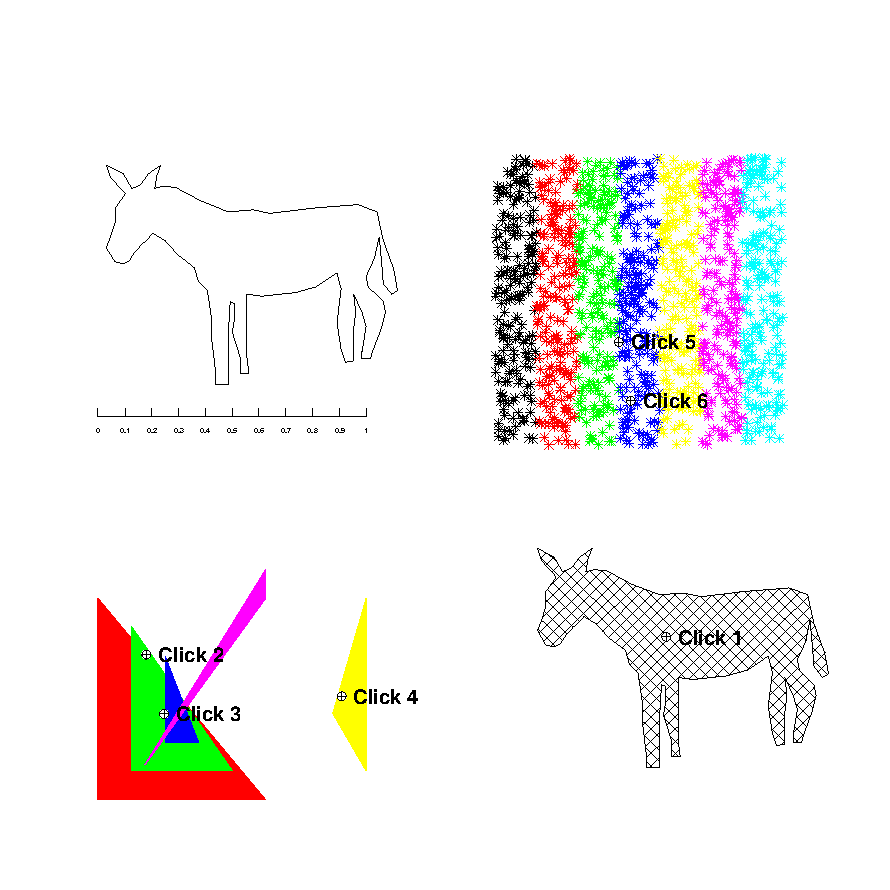
\includegraphics[width=\linewidth]{pick.eps}
\end{center}
\caption{A structured picture}
\label{PICK}
\end{figure}

